
\subsection{Answers}
\begin{table}[htb]%
\begin{center}%
\caption{Q20: When you call an MPI routine, how often do you check the error code of the MPI routine  (excepting MPI-IO)?}%
\label{tab:Q20-ans}%
\begin{tabular}{l|l|r}%
\hline%
Choice & Abbrv. & \# Answers \\%
\hline%
{\small I rely on the default ‘Errors abort’ err$\cdots$} & Default & 177 (21.8\%) \\%
Always & Always & 108 (13.3\%) \\%
Mostly & Mostly & 155 (19.1\%) \\%
Sometimes & Sometimes & 259 (31.9\%) \\%
Never & Never & 112 (13.8\%) \\%
\hline%
\multicolumn{2}{c}{total} & 811 \\%
\hline%
\end{tabular}%
\end{center}%
\end{table}%


\begin{figure}[htb]
\begin{center}
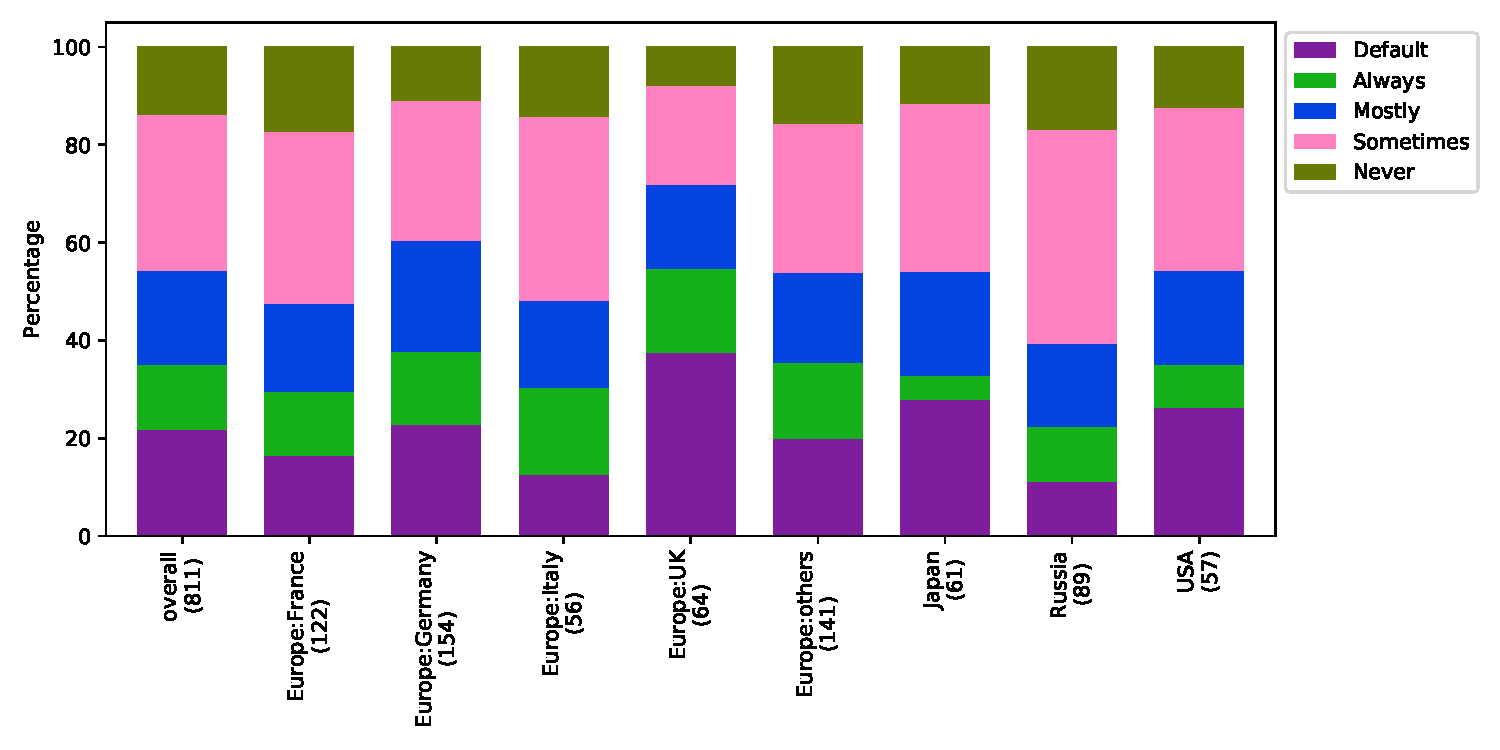
\includegraphics[width=10cm]{../pdfs/Q20.pdf}
\caption{Simple analysis: Q20}
\label{fig:Q20}
\end{center}
\end{figure}

The 'default' and 'never' are theoretically have the same meaning. I
wonder how they distingushed them?

Excepting UK, the 'sometimes' answer dominates. Do they check errors
only at critical points or just fitfully?

In Japan, the 'always' answer has the smallest percentage.  Where is
the uprightness?
